\documentclass[12pt,a4paper, spanish]{article}
% Sacar draft para que aparezcan las imagenes.
% Opciones: 12pt, 10pt, 11pt, landscape, twocolumn, fleqn, leqno...
% Opciones de clase: article, report, letter, beamer...

% Paquetes:
% =========
\usepackage[headheight=110pt, top = 2cm, bottom = 2cm, left=1cm, right=1cm]{geometry} %modifico márgenes
\usepackage[T1]{fontenc} % tildes
\usepackage[utf8]{inputenc} % Para poder escribir con tildes en el editor.
\usepackage[english]{babel} % Para cortar las palabras en silabas, creo.
\usepackage[ddmmyyyy]{datetime}
\usepackage{amsmath} % Soporte de mathmatics
\usepackage{amssymb} % fuentes de mathmatics
\usepackage{array} % Para tablas y eso
\usepackage{caption} % Configuracion de figuras y tablas
\usepackage[dvipsnames]{xcolor} % Para colorear el texto: black, blue, brown, cyan, darkgray, gray, green, lightgray, lime, magenta, olive, orange, pink, purple, red, teal, violet, white, yellow.
\usepackage{graphicx} % Necesario para poner imagenes
\usepackage{enumitem} % Cambiar labels y más flexibilidad para el enumerate
\usepackage{multicol} 
\usepackage{tikz} % para graficar
\usepackage{cancel} % cancelar fórmulas
\usepackage{titlesec} % para editar titulos y hacer secciones con formato a medida
\usepackage{ulem}
\usepackage{centernot} % tacha cosas
\usepackage{bbding} % símbolos de donde uso FiveStar
\usepackage{skull} % símbolos de donde uso Skull
\usepackage{soul} % Para tachar texto en text y math mode

% \usepackage{lipsum} % dummy text

% para hacer los graficos tipo grafos
\usetikzlibrary{shapes,arrows.meta, chains, matrix, calc, trees, positioning, fit}
\usetikzlibrary{external}

\setlength{\parindent}{0pt} % Para que no haya indentación en las nuevas líneas.

% Definiciones y macros para que se me haga
% más ameno el codeo.
% Definiciones y nuevos comandos:def
% =============
% Conjuntos
\DeclareMathOperator{\partes}{\mathcal P}
\DeclareMathOperator{\relacion}{\,\mathcal{R}\,}
\DeclareMathOperator{\norelacion}{\,\cancel{\relacion}\,}
\DeclareMathOperator{\universo}{\mathcal U}
\DeclareMathOperator{\reales}{\mathbb R}
\DeclareMathOperator{\naturales}{\mathbb N}
\DeclareMathOperator{\enteros}{\mathbb Z}
\DeclareMathOperator{\racionales}{\mathbb Q}
\DeclareMathOperator{\irracionales}{\mathbb I}
\DeclareMathOperator{\complejos}{\mathbb C}


\DeclareMathOperator{\K}{\mathbb K} % cuerpo K
\DeclareMathOperator{\vacio}{\varnothing}
\DeclareMathOperator{\union}{\cup}
\DeclareMathOperator{\inter}{\cap}
\DeclareMathOperator{\diferencia}{\ \setminus \ }
\DeclareMathOperator{\y}{\land}
\def\o{\lor}
\def\neg{\sim}

\def\entonces{\Rightarrow}
\def\noEntonces{\centernot\Rightarrow}

\def\sisolosi{\iff} % largo
\def\sii{\Leftrightarrow} % corto

\def\clase{\overline}
\def\ord{\text{ord}}


\def\existe{\,\exists\,}
\def\noexiste{\,\nexists\,}
\def\paratodo{\ \, \forall}
\def\distinto{\neq}
\def\en{\in}
\def\talque{\;/\;}

% =====
\def\qvq{\text{ quiero ver que }}

%funciones
\DeclareMathOperator{\dom}{Dom}
\DeclareMathOperator{\cod}{Cod}
\def\F{\mathcal F}
\def\comp{\circ}
\def\inv{^{-1}}
\def\infinito{\infty}

% Llaves, paréntesis, contenedores
\newcommand{\llave}[2]{ \left\{ \begin{array}{#1} #2 \end{array}\right. }
\newcommand{\llaveInv}[2]{ \left\} \begin{array}{#1} #2 \end{array}\right. }
\newcommand{\llaves}[2]{ \left\{ \begin{array}{#1} #2 \end{array} \right\} }
\newcommand{\matriz}[2]{\left( \begin{array}{#1} #2 \end{array} \right)}
\newcommand{\deter}[2]{\left| \begin{array}{#1} #2 \end{array} \right|}
\newcommand{\lista}[2][(1)]{\begin{enumerate}[\bf #1]\setlength\itemsep{-0.6ex} #2 \end{enumerate}}
\newcommand{\listal}[2][-0.6ex]{\begin{enumerate}[\bf(a)]\setlength\itemsep{#1} #2 \end{enumerate}}

% naturales
\newcommand{\sumatoria}[2]{\sum\limits_{#1}^{#2}}
\newcommand{\productoria}[2]{\prod\limits_{#1}^{#2}}
\newcommand{\kmasuno}[1]{\underbrace{#1}_{k+1\text{-ésimo}}}
\newcommand{\HI}[1]{\underbrace{#1}_{\text{HI}}}

% % enteros
\def\divideA{\, | \,}
\def\noDivide{\centernot\divideA}
\def\congruente{\, \equiv \,}
\newcommand{\congruencia}[3]{#1 \equiv #2 \;(#3)}
\newcommand{\noCongruencia}[3]{#1 \not\equiv #2 \;(#3)}
\newcommand{\conga}[1]{\stackrel{(#1)}{\congruente}}
\newcommand{\divset}[2]{\mathcal{D}(#1) = \set{#2}}
\newcommand{\divsetP}[2]{\mathcal{D_+}(#1) = \set{#2}}
\newcommand{\ub}[2]{ \underbrace{\textstyle #1}_{\mathclap{#2}} }
\newcommand{\ob}[2]{ \overbrace{\textstyle #1}^{\mathclap{#2}} }
\def\cop{\, \perp \, }

% complejos
\DeclareMathOperator{\re}{Re}
\DeclareMathOperator{\im}{Im}
\DeclareMathOperator{\argumento}{arg}
\newcommand{\conj}[1]{\overline{#1}}

% Polinomios
\DeclareMathOperator{\cp}{cp}
\DeclareMathOperator{\gr}{gr}
\DeclareMathOperator{\mult}{mult}
\newcommand{\divPol}[2]{\polylongdiv[style=D]{#1}{#2}}
\newcommand{\mcd}[2]{\polylonggcd{#1}{#2}}


% =====
% Miscelanea
% =====
\def\ot{\leftarrow}
\newcommand{\estabien}{{\color{blue} Consultado, está bien. \checkmark}}
\newcommand{\hacer}{
  {\color{red!80!black}{\Large \faIcon{radiation} Falta hacerlo!}}\par
  {\color{black!70!white}
    \small Si querés mandarlo: Telegram $\to$ \href{https://t.me/+1znt2GV1i8cwMTNh}{\small\faIcon{telegram}},
    o  mejor aún si querés subirlo en \LaTeX $\to$ \href{https://github.com/nad-garraz/algebraUno}{\small \faIcon{github}}.
  }\par
}

\newcommand{\Hacer}{{\color{black!30!red}\Large Hacer!}}
\def\Tilde{\quad\checkmark}
\def\ytext{\text{ y }}
\def\otext{\text{ o }}

% Estrellita para hacer llamadas de atención, viene en divertidos colores
% para coleccionar.
\newcommand{\llamada}[1]{
  \textcolor{
    \ifcase \numexpr#1 mod 6\relax
      cyan\or magenta\or OliveGreen\or YellowOrange\or Cerulean\or Violet\or Purple\or
    \fi
  }
  {\text{\FiveStar}^{\scriptscriptstyle#1}}
}


% separadores
\def\separador{\par\medskip\rule{\linewidth}{0.4pt}\par\medskip}
\def\separadorCorto{\par\medskip\rule{0.5\linewidth}{0.4pt}\par\medskip}


% Colores
\newcommand{\red}[1]{\textcolor{red}{#1}}
\newcommand{\green}[1]{\textcolor{OliveGreen}{#1}}
\newcommand{\blue}[1]{\textcolor{Cerulean}{#1}}
\newcommand{\cyan}[1]{\textcolor{cyan}{#1}}
\newcommand{\yellow}[1]{\textcolor{YellowOrange}{#1}}
\newcommand{\magenta}[1]{\textcolor{magenta}{#1}}
\newcommand{\purple}[1]{\textcolor{purple}{#1}}

% Conjuntos entre llaves y paréntesis
% te ahorrás escribir los \left y \right, así dejando el código más legible.
\newcommand{\set}[1] { \left\{ #1 \right\} }
\newcommand{\parentesis}[1]{ \left( #1 \right) }

% Stackrel text. Es para ahorrarse ecribir el \text
\newcommand{\stacktext}[2]{ \stackrel{\text{#1}}{#2} }

% Dado que muchas veces ponemos cosas sobre un signo '='
%  acá está el comando para escribir \igual{arriba}[abajo] con texto!
\NewDocumentCommand{\igual}{m o}{
  \IfNoValueTF{#2}{
    \overset{\mathclap{\text{#1}}}=
  }{
    \overset{\mathclap{\text{#1}}}{\underset{\mathclap{\text{#2}}}=}
  }
}
% Dado que muchas veces ponemos cosas sobre un signo '='
%  acá está el comando para escribir \igual{arriba}[abajo] con texto!
\NewDocumentCommand{\mayorIgual}{m o}{
  \IfNoValueTF{#2}{
    \overset{\mathclap{\text{#1}}}\geq
  }{
    \overset{\mathclap{\text{#1}}}{\underset{\mathclap{\text{#2}}}\geq}
  }
}
% Dado que muchas veces ponemos cosas sobre un signo '='
%  acá está el comando para escribir \igual{arriba}[abajo] con texto!
\NewDocumentCommand{\menorIgual}{m o}{
  \IfNoValueTF{#2}{
    \overset{\mathclap{\text{#1}}}\leq
  }{
    \overset{\mathclap{\text{#1}}}{\underset{\mathclap{\text{#2}}}\leq}
  }
}


%=======================================================
% Comandos con flechas extensibles.
%=======================================================
% *Flechita* extensible con texto {arriba} y [abajo] 
\NewDocumentCommand{\flecha}{m o}{%
  \IfNoValueTF{#2}{%
    \xrightarrow[]{\text{#1}}
  }{
    \xrightarrow[\text{#2}]{\text{#1}}
  }
}
% *Si solo si* extensible con texto {arriba} y [abajo] 
\NewDocumentCommand{\Sii}{m o}{%
  \IfNoValueTF{#2}{%
    \xLeftrightarrow[]{\text{#1}}
  }{
    \xLeftrightarrow[\text{#2}]{\text{#1}}
  }
}

% *Si solo si* extensible con texto {arriba} y [abajo] 
\NewDocumentCommand{\Entonces}{m o}{%
  \IfNoValueTF{#2}{%
    \xRightarrow[]{\text{#1}}
  }{
    \xRightarrow[\text{#2}]{\text{#1}}
  }
}

%=======================================================
% fin comandos con flechas extensibles.


% como el stackrel pero también se puede poner algo debajo
\newcommand{\taa}[3]{ % [t]exto [a]rriba y [a]bajo
  \overset{\mathclap{#1}}{\underset{\mathclap{#2}}{#3}}
}

%Update time
\def\update{
  actualizado: \today
}


%=======================================================
% sección ejercicio con su respectivo formato y contador
%=======================================================
\newcounter{ejercicio}[section] % contador que se resetea en cada sección
\renewcommand{\theejercicio}{\arabic{ejercicio}} % el contador es un número arabic
\newcommand{\ejercicio}{%
  \stepcounter{ejercicio}% incremento en uno
  \titleformat{\section}[runin]{\bfseries}{\theejercicio}{1em}{}%
  \section*{\theejercicio.}\labelEjercicio{ej:\theejercicio}
}

% Label y refencia para ejercicio hay alguna forma más elegante de hacer esto?
\newcommand{\labelEjercicio}[1]{
  \addtocounter{ejercicio}{-1} % counter - 1
  \refstepcounter{ejercicio} % referencia al anterior y luego + 1
  \label{#1}}
\newcommand{\refEjercicio}[1]{{ \bf\ref{#1}.}}

\def\fueguito{{\color{orange}{\faIcon{fire}}}}
\newcounter{ejExtra}[section] % contador que se resetea en cada sección
\renewcommand{\theejExtra}{\arabic{ejExtra}} % el contador es un número arabic
\newcommand{\ejExtra}{%
  \stepcounter{ejExtra}% incremento en uno
  \titleformat{\section}[runin]{\bfseries}{\theejExtra}{1em}{}%
  % Es como una sección. Le pongo un ícono, luego el número del ejercicio con la etiqueta para poder
  % linkearlo en el índice u otro lugar.
  % con \ref{ejExtra:{numero del ejercicio}} es que salto al ejercicio.
  \section*{\fueguito\theejExtra.}\labelEjExtra{ejExtra:\theejExtra}
}

% Label y refencia para ejercicio hay alguna forma más elegante de hacer esto?
\newcommand{\labelEjExtra}[1]{
  \addtocounter{ejExtra}{-1} % counter - 1
  \refstepcounter{ejExtra} % referencia al anterior y luego + 1
  \label{#1} % etiqueta para cada ejercicio extra
}
% Con esto llamos al ejercicio extra
\newcommand{\refEjExtra}[1]{
  {\fueguito\bf\ref{#1}.}
}

%=======================================================
% fin sección ejercicio con su respectivo formato y contador
%=======================================================

\newenvironment{enunciado}[1]{ % Toma un parametro obligatorio: \ejExtra o \ejercicio 
  \separador % linea sobre el enunciado
  \begin{minipage}{\textwidth}
    #1
    }% contenido
    {
  \end{minipage}
    \separadorCorto % linea debajo del enunciado
}



\begin{document}

% Info para armar título.
\title{Práctica 6 de álgebra 1} % título
\author{Comunidad algebraica} % autor
\date{last update: \today} % Cambiar de ser necesario
\maketitle  % para que aprezca el título en el documento


%=========================
% Un poco de teoría
%=========================
\textit{\underline{Raíces de un número complejo: }}

\begin{itemize}[label= \tiny \faIcon{meh}]

  \item \hypertarget{teoria-6:tablita}{Tablita de ángulos \textit{agradables}}:

        \begin{minipage}{0.5\textwidth}
          $$
            \begin{array}{|c|c|c|c|c|c|}
              \hline
                    \theta       & \red{0} & \color{orange}{\frac{\pi}{6}}      & \green{\frac{\pi}{4}}      & \color{blue}{\frac{\pi}{3}}      & \purple{\frac{\pi}{2}} \\ \hline
              \sin(\theta) & 0 & \frac{1}{2}        & \frac{\sqrt{2}}{2} & \frac{\sqrt{3}}{2} & 1             \\ \hline
              \cos(\theta) & 0 & \frac{\sqrt{3}}{2} & \frac{\sqrt{2}}{2} & \frac{1}{2}        & 1             \\ \hline
            \end{array}
          $$
                {\small
                \href{https://www.youtube.com/watch?v=83gdQe0Ij5k}{Clickea para está \textit{simpatética} forma de recordarlo:
                \purple{\faIcon{music}} um, dois, três, três, dois, um, todo mundo sobre 2...\purple{\faIcon{music}}}}
        \end{minipage}
        \begin{minipage}{0.5\textwidth}
          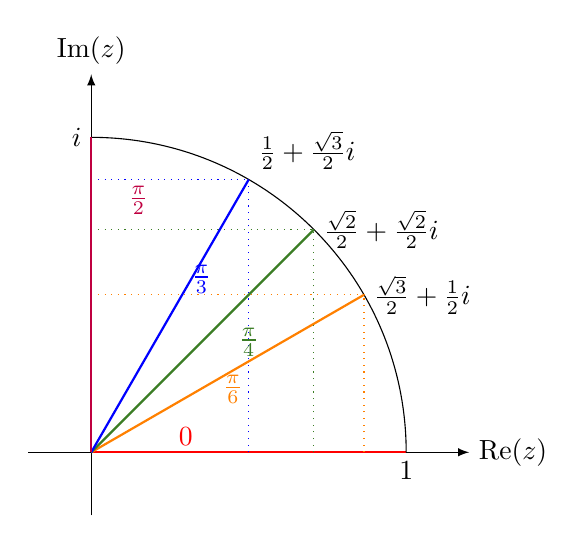
\begin{tikzpicture}[scale=4]
            % Draw the main coordinate axes
            \draw[-latex] (-0.2,0) -- (1.2,0) node[right] {$\re(z)$};
            \draw[-latex] (0,-0.2) -- (0,1.2) node[above] {$\im(z)$};

            \draw[red,thick] (0,0) -- (1,0);
            \draw[thin] (1,0) arc (0:90:1);

            \draw[orange,thick] (0,0) -- ({sqrt(3)/2},{1/2});
            \draw[orange,dotted] ({sqrt(3)/2},0) -- ({sqrt(3)/2},{1/2});
            \draw[orange,dotted] (0,{1/2}) -- ({sqrt(3)/2},{1/2});

            \draw[OliveGreen,thick] (0,0) -- ({1/sqrt(2)},{1/sqrt(2)});
            \draw[OliveGreen,dotted] ({1/sqrt(2)},0) -- ({1/sqrt(2)},{1/sqrt(2)});
            \draw[OliveGreen,dotted] (0,{1/sqrt(2)}) -- ({1/sqrt(2)},{1/sqrt(2)});

            \draw[blue,thick] (0,0) -- ({1/2},{sqrt(3)/2});
            \draw[blue,dotted] ({1/2},0) -- ({1/2},{sqrt(3)/2});
            \draw[blue,dotted] (0,{sqrt(3)/2}) -- ({1/2},{sqrt(3)/2});

            \draw[purple,thick] (0,0) -- (0,1);

            \node[red] at (0.3,0.05) {$0$};
            \node[orange] at (0.45,0.2) {$\frac{\pi}{6}$};
            \node[OliveGreen] at (0.5,0.35) {$\frac{\pi}{4}$};
            \node[blue] at (0.35,0.55) {$\frac{\pi}{3}$};
            \node[purple] at (0.15,0.8) {$\frac{\pi}{2}$};

            \node[below] at (1,0) {$1$};
            \node[right] at ({sqrt(3)/2},{1/2}) {$\frac{\sqrt{3}}{2} + \frac{1}{2}i$};
            \node[right] at ({1/sqrt(2)},{1/sqrt(2)}) {$\frac{\sqrt{2}}{2} + \frac{\sqrt{2}}{2}i$};
            \node[above right] at ({1/2},{sqrt(3)/2}) {$\frac{1}{2} + \frac{\sqrt{3}}{2}i$};
            \node[left] at (0,1) {$i$};
          \end{tikzpicture}
        \end{minipage}

  \item Sean $z, w \en \complejos -\set{0}$, $z = r_z e^{\theta_z i}$ y $w = r_w e^{\theta_w i }$ con $r_z,\, s_w \en \reales_{>0}$
        y $\theta_z,\, \theta_w \en \reales$.\par
        Entonces $z = w
          \Sii{\red{!!}}
          \llave{l}{
            r_z = r_w \\
            \theta_z = \theta_w + 2 k \pi,\ \text{para algún } k \en \enteros
          }$
  \item raíces $n$-esimas: $w^n = z
          \Sii{\red{!!}}
          \llave{l}{
            (r_w)^n = r_z \\
            \theta_w \cdot n = \theta_z + 2 k \pi \quad \text{para algún $k\en \enteros$}
          }$\par
        De donde se obtendrán $n$ raíces distintas:
        $$
          w_k = z_w e^{\theta_{w_k} i}, \text{ donde } r_w = \sqrt[n]{r_z} \ytext
          \theta_{w_k} = \frac{\theta_z}{n} + \frac{2k\pi}{n} = \frac{\theta_z + 2k\pi}{n}
        $$
        \red{Entender bien como sacar raíces $n$-ésimas es importantísimo para toda la guía de complejos y la próxima de polinomios}.
\end{itemize}

\underline{\textit{Grupos $G_n$:}}

\begin{itemize}[label=\color{gray} \tiny \faIcon{smile}]
\item $G_n = \set{w \en \complejos / w^n = 1} = \set{e^{\frac{2k \pi}{n} i}\ :\ 0\leq k \leq n-1}$
%==========================
% Macro para reducir los gráficos
\newcommand{\unitcircle}[1]{
  \begin{tikzpicture}[baseline=0, scale=1, every node/.style={font=\tiny}]
    \draw[ultra thin,->,gray] (-1.5,0) -- (1.8,0) node[below] {Re};
    \draw[ultra thin,->,gray] (0,-1.5) -- (0,1.5) node[right] {Im};
    \draw[ultra thin] (0,0) circle (1);
    \foreach \x in {0,...,#1} {
        \ifnum \x < #1 {
              \filldraw (\x*360/#1:0.8) node {$\x$};
              \filldraw (\x*360/#1:1) circle (1pt);
              \filldraw (\x*360/#1:1.4) node {$e^{i \frac{2\pi}{#1} \cdot \x}$};
              \draw[thick, Cerulean] (\x*360/#1:1) -- ({(\x+1)*360/#1}:1);
            }
        \fi
      }
  \end{tikzpicture}
}
% Fin macros
%================================

\begin{multicols}{2}
  \begin{enumerate}[label={($n$=\arabic*)}]
    \item $w = 1$
    \item $w = \pm 1$
    \item \unitcircle{3}
    \item \unitcircle{4}
    \item \unitcircle{5}
    \item \unitcircle{6}
    \item \unitcircle{7}
    \item \unitcircle{8}
    \item \unitcircle{9}
    \item \unitcircle{10}
  \end{enumerate}
\end{multicols}
Notar que:
\begin{itemize}
  \item Si $n$ es par el grupo tiene al $-1$.
  \item Toda raíz compleja tiene a su conjugado complejo.
  \item Para ir de un punto a otro, se lo múltiplica por $e^{i \theta}$ eso \textit{rota} al número en $\theta$
        respecto al origen.
\end{itemize}

\item $(G_n, \cdot)$ es un grupo abeliano, o conmutativo.
\begin{itemize}
  \item $\paratodo w, z \en G_n, w z = z  w \text{ y } z m \en G_n$.

  \item $1 \en G_n,\ w \cdot 1 = 1 \cdot w = w \qquad \paratodo w \en G_n$.

  \item $w \en G_n \entonces \existe w^{-1} \en G_n,\ w \cdot w^{-1} = w^{-1}\cdot w = 1$
        \begin{itemize}
          \item $\conj w \en G_n,\ w \cdot \conj w = |w|^2 = 1 \entonces \conj w = w^{-1}$
        \end{itemize}
\end{itemize}

\item \textit{Propiedades: $w \en G_n$}
\begin{itemize}
  \item $m \en \enteros$ y $n \divideA m \entonces w^m = 1$.

  \item $\congruencia{m}{m'}{n} \entonces w^m = w^{m'}\quad (w^m = w^{r_n(m)})$

  \item $n \divideA m \sisolosi G_n \subseteq G_m$

  \item $G_n \inter G_m = G_{(n:m)}$

  \item La suma de una raíz $w$ de $G_n$:
        $\sumatoria{k=0}{n-1}w^k = \frac{w^n -1}{w -1} = 0$ si $w \distinto 1$
\end{itemize}


%=========================
% Fin un poco de teoría
%=========================

\newpage % página nueva

%=========================
% Ejercicios extras, parciales, etc.
%=========================
\subsubsection*{Ejercicios extras:}

\foreach \x in {1,2} {
		\input{./ejercicios-6-extra/ej-extra-\x-6.tex}
	}

%=========================
% Fin ejercicios extras, parciales, etc.
%=========================

\newpage % página nueva

%=========================
% Ejercicios guia
%=========================

\subsubsection*{Ejercicios de la guía:}
\setcounter{ejercicio}{0} % Reset el counter de \ejercicio

\foreach \x in {1,...,15} {
		\input{./ejercicios-6/ej-\x-6.tex}
	}
%=========================
% Fin ejercicios guia
%=========================

\end{document}
